\documentclass[a4paper,12pt]{scrartcl}

\usepackage{amsmath}
\usepackage{scrextend}
\usepackage{graphicx}
\usepackage[T1]{fontenc}
\usepackage[ngerman]{babel}
\usepackage[colorlinks,
pdfpagelabels,
pdfstartview = FitH,
bookmarksopen = true,
bookmarksnumbered = true,
linkcolor = black,
plainpages = false,
hypertexnames = false,
citecolor = black] {hyperref}


\begin{document}

\title{Paläontologie}
\maketitle



\begin{itemize}



\section{Aufgabenbereich} \label{sec:Aufgabenbereich}
\item Taxonomie fossieler Lebewesen, inc. Spurenfossilien 
\item Wechselwirkungen mit der Parläo-umwelt: Palökologie
\item Entwicklung in der Zeit: Phylogenie und Biostrategraphie, Geobiologie, Paläobiologie
\item Analyse natürlicher biologischer Langzeitexperimente



\section{Fossilien} \label{sec:Fossilien}

\item Körperfossilien: versteinerte Überreste von Organismen
\item lebende Fossilien: quastenflosser, Lingula; Lebewesen, die in ihrer Morphologie unverändert sind
\item Chemofossilien: organische Verbindungen, welche bestimmten Organismengruppen zugeordnet werden kann; z.B Biomarker, Farbstoffe oder Pigmente
\item Spurenfossilien (Ichnofossilien): z.B. Fußspuren, Bissspuren; setzt Aktivität des Lebewesens voraus

\newpage

\section{Taphonomie} \label{sec:Taphonomie}

\item Beschäftigt sich mit den Prozessen vom versterben bis zum Fossil

\begin{addmargin}[20mm]{0mm}
\item studiert den Zerfall von Organsimen und deren Ablagerung/Einbettung
\item studiert Diagnese von eingebetteten Organismen/Communities
\item versucht Biozönose (Lebensgemeinschaft) und Tanatoönosezu (Todesgemeinschaft) rekonstruieren
\end{addmargin}

\item liefert wichtige Infos über Physikalische Parameter: z.B Akkumulationsraten, Strömungen, Auflösung etc.

\section{Möglichhkeiten zu sterben} \label{sec:Möglichkeiten zu sterben}

\item natürliches Altern
\item Nahrungsmangel
\item Fallen:

\begin{addmargin}[20mm]{0mm}
1. Bernstein \\
2. Karstschlotten (natürliche Fallgruben) \\
3. Teergruben
\end{addmargin}

\item Prädation (Räuber-Beute-Spuren z.B Bissspuren)
\item schlechte Ernährung
\item Parasitismus
\item Inkrustation (Bewuchs)
\item Verschüttung
\item Umweltkatastrophen/Wechselwirkungen
\end{itemize}


%VLS fehlt

\section{Erhaltungszustände}

\textbf{Weichteil und Gewebeerhaltung}

\begin{enumerate}
\item Mumie
\item Mumien-Pseudomorphose
\item Weichkörperausdrücke
\item Weichkörpermineralisierung
\item Farberhaltung
\end{enumerate}
Weichteilmineralisierung zählt zu Weichteilerhaltung
\textbf{Hartteilerhaltung}

\begin{enumerate}
\item oreginaler Zustand
\item Steinkern, Prägesteinkern\\
\begin{itemize}
\item Steinkern: Innenabdruck 
\item Prägesteinkern: Merkmale der äußeren Schale werden auf Steinkern geprägt, nachdem die Schale weggelöst wurde
\end{itemize}
\item Abdruck
\item Pseudomorphose (nicht mehr die richtige Mumie, sondern substituierter Rest.)
\end{enumerate}
Bioimmuration (Inkrustation): z.B Abdruck von Amunit auf Muschelschale

\textbf{Prägesteinkern}\\
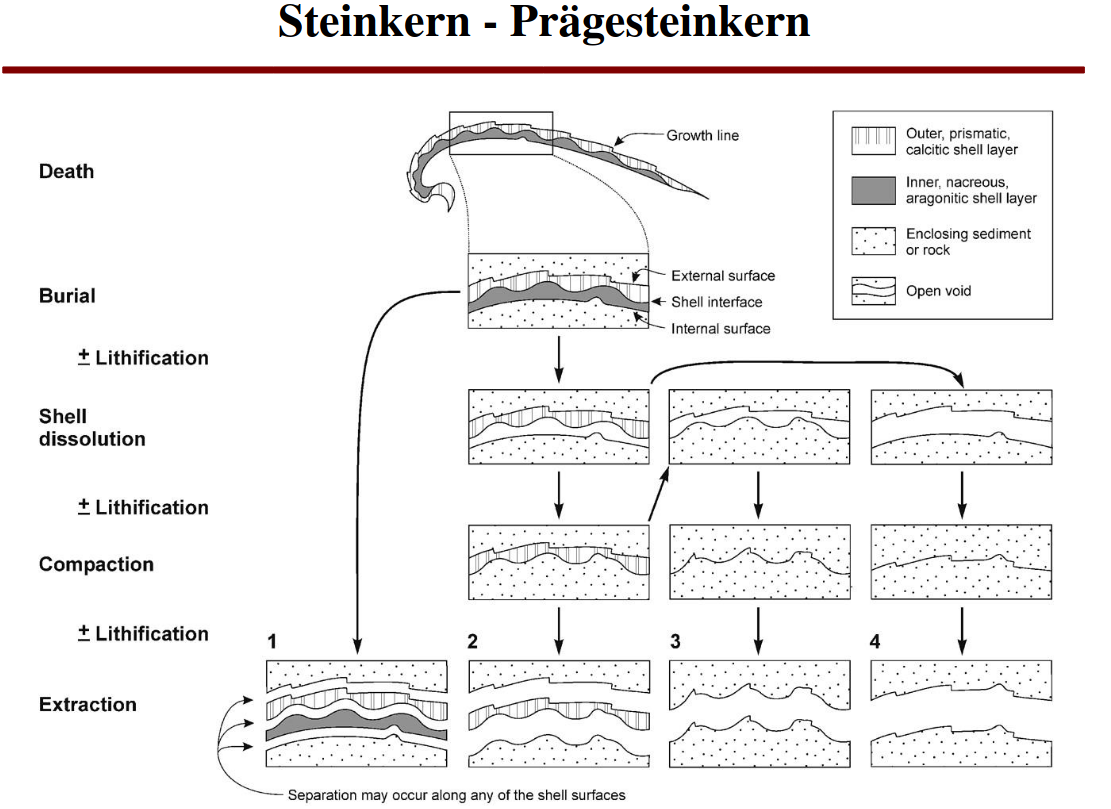
\includegraphics[width=0.8\textwidth]{/home/joni/Schreibtisch/Uni/Mittschriften/Parlo/Bilder/Steinkern}\\
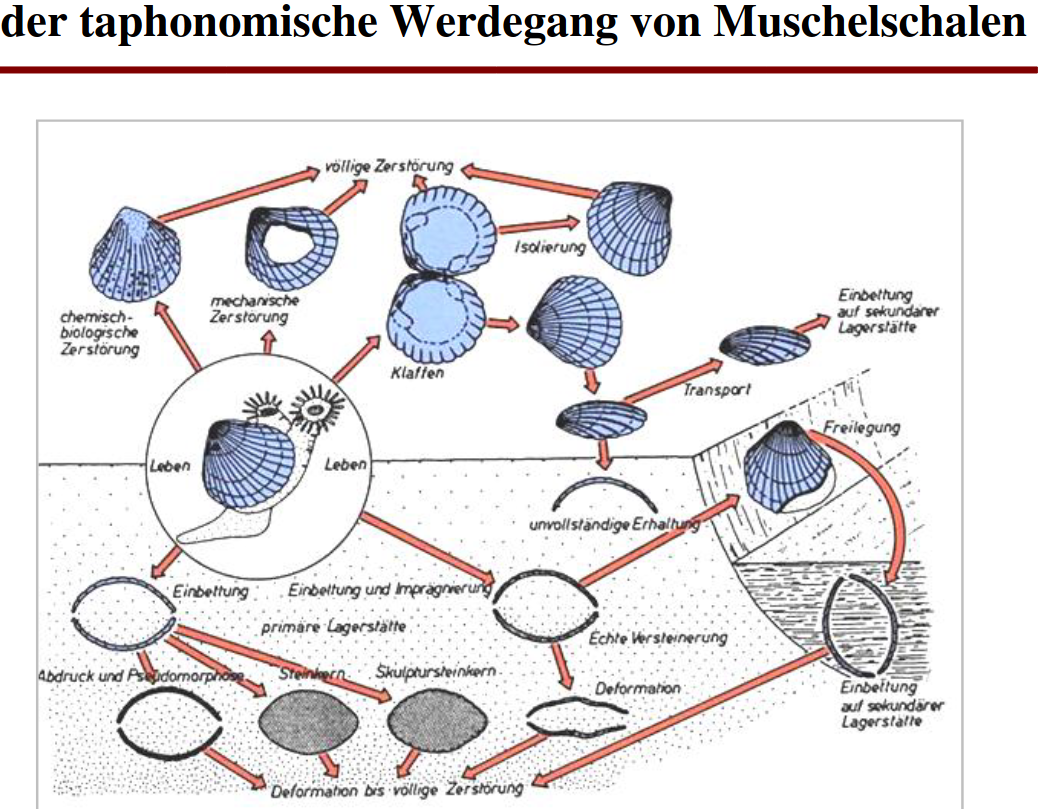
\includegraphics[width=0.8\textwidth]{/home/joni/Schreibtisch/Uni/Mittschriften/Parlo/Bilder/Zusammenfassung}\\

Bioimmuration (Inkrustation): z.B Abdruck von Amunit auf Muschelschale

\textbf{Prozesse nach der Einbettung}\\
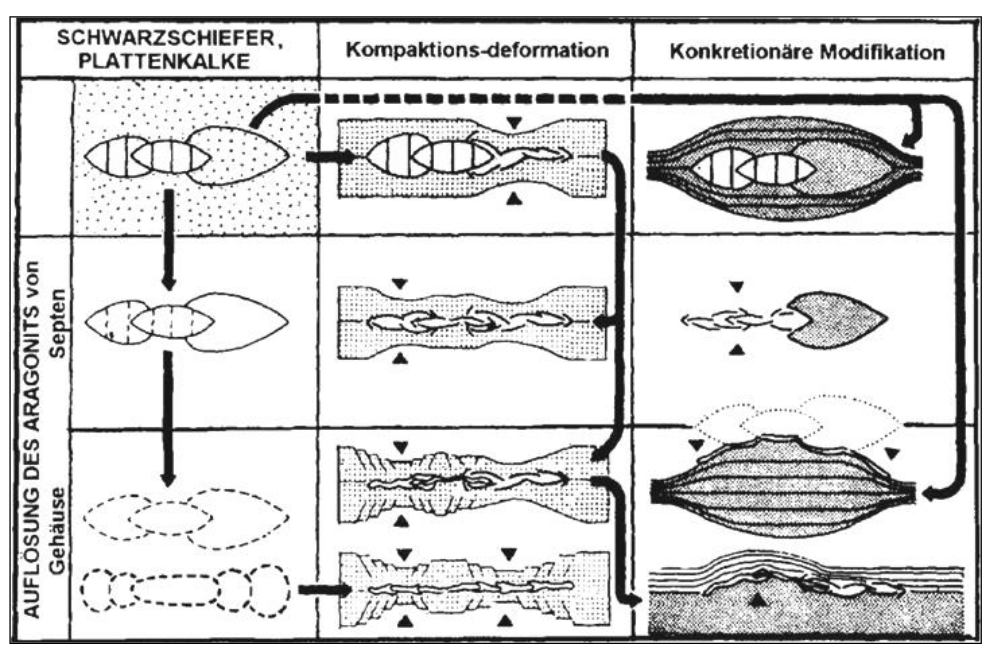
\includegraphics[width=0.8\textwidth]{/home/joni/Schreibtisch/Uni/Mittschriften/Parlo/Bilder/Kopaktion}\\

\newpage
\section{Fossiellagerstätten}
\begin{enumerate}
\item Kenzentrationslagerstätten
\begin{itemize}
\item Kondensation (kaum Sedimentation)
\item Konzentration (z.B. Höhlen)
\end{itemize}
\item Konservatlagerstätten
\begin{itemize}
\item Stagnation (z.B. anoxische, euxinische, salinare Wässer)
\item Verschüttungslagerstätten (Turbidite, Tempesite)
\item Erhaltungsfallen (Rancho La Brea)
\end{itemize}
\end{enumerate}

Grundvoraussetzung: wenig Sauerstoff im Boden\\
Entstehung anoxischer/ euxinischen Wässern: \\
\begin{itemize}
\item sehr viel Leben, viel Organische Zeretzung am Boden fürht zu Sauerstoffverbrauch.
\end{itemize}

\subsection{fossil record}
kann nicht vollständig sein\\
Lücken durch nicht fossilisierbare Lebewesen\\
Lebewesen aus verschiedensten Zeitaltern im gleichen Sediment\\
Verlust der kleinen fossilien (wird übersehen oder erodiert leichter)


\section{Parläophysiologie}
- befasst sich mit den physikalischen und biochemischen Vorgängen von Zellen, Geweben und Organen sowie ihrem Zusammenwirken im Gesamtorganismus „Lebensvorgänge“, soweit dies überhaupt für fossile Organismen rekonstruierbar ist\\
- wesentliche Grundlage zur Rekonstruktion von Ablagerungs und Lebensräumen
- wichtig für palökolologische Betrachtungsweisen
- Beeinflussung durch äußere



\subsection{Ernährungsweise}
\begin{enumerate}
\item Autotrophie\\
-Ernährung aus anorg. Grundstoffen
\item Mikrophagie
-Ernährung aus tierischen/pflanzlichen Plankton
\item Herbi/Carnivorie
\item Omnivorie, Saprophragie\\
-Alles/Abfallfresser
\end{enumerate}

\subsubsection{Chem-Autotrophie}
Energiegewinnung durch Oxidation von Fe, S, N, $NH_3$\\
bei Bakterien oder Archeae z.B an Tiefseesmokern\\










\end{document}